\documentclass[11pt]{article}

% ==== PACKAGES ==== %
% \usepackage{fullpage}
\usepackage{amsmath,amssymb,amsthm}
\usepackage{epic}
\usepackage{eepic}
\usepackage{hyperref}
\usepackage{listings}
\usepackage{float}
\usepackage{graphicx}
\usepackage{fancyhdr}
\usepackage{color}
\usepackage{bbm}
\usepackage[letterpaper, margin=1in]{geometry}

% ==== MARGINS ==== %
% \pagestyle{empty}
% \setlength{\oddsidemargin}{0in}
% \setlength{\textwidth}{6.8in}
% \setlength{\textheight}{9.5in}

\pagestyle{fancy}
\fancyhf{}
\rhead{ASEN 5044}
\lhead{Homework 1}
\rfoot{Page \thepage}


\newtheorem*{solution*}{Solution}
\newtheorem{lemma}{Lemma}[section]
\newtheorem{theorem}[lemma]{Theorem}
\newtheorem{claim}[lemma]{Claim}
\newtheorem{definition}[lemma]{Definition}
\newtheorem{corollary}[lemma]{Corollary}
\lstset{moredelim=[is][\bfseries]{[*}{*]}}

% ==== DOCUMENT PROPER ==== %
\begin{document}

\thispagestyle{empty}

% --- Header Box --- %
\newlength{\boxlength}\setlength{\boxlength}{\textwidth}
\addtolength{\boxlength}{-4mm}

\begin{center}\framebox{\parbox{\boxlength}{\bf
      Statistical Estimation \hfill Homework 2\\
      ASEN 5044 Fall 2018 \hfill Due Date: Sep 20, 2018\\
      Name: Andrew Kramer \hfill PhD Student
}}
\end{center}

\section*{Exercise 1}
In the game of blackjack, the player is initially dealt two cards from a deck of ordinary playing cards. Without going into all the game's details, it is enough to know the best possible hand for a player to receive on the initial deal is a combination of an ace of any suit and any face card or ten. What is the probability that a player will be dealt this combination?

\subparagraph*{}
The number of ways a single player can be dealt a blackjack (assuming there is only one player) is ${4\choose1}{16\choose1} = 64$. So the number of events in our event space (which we'll call $A$) is 64. The total number of ways to deal 2 cards to that player is ${52\choose2} = 1326$. So, the number of events in the whole sample space is 1326. the probability of a single player being dealt a blackjack is therefore
\begin{equation*}
	\frac{N_A}{N} = \frac{{4\choose1}}{{16\choose1}} = \frac{64}{1326} = 0.048
\end{equation*}

\section*{Exercise 2}
Discrete and random variables $X$ and $Y$ can each take on integer values 1, 3, and 5. The joint probability table of $X$ and $Y$ is given below.

\begin{table}[h!]
  \begin{center}
    \caption{Joint Probabilities}
    \label{tab:table1}
    \begin{tabular}{c|c|c|c} % <-- Alignments: 1st column left, 2nd middle and 3rd right, with vertical lines in between
      X & Y=1 & Y=3 & Y=5\\
      \hline
      1 & 1/18 & 1/18 & 1/18 \\
      3 & 1/18 & 1/18 & 1/6 \\
      5 & 1/18 & 1/6 & 1/3\\
    \end{tabular}
  \end{center}
\end{table}

\subsection*{Problem (a)}
Are the random variables $X$ and $Y$ independent?

\subparagraph*{}
No, the table clearly shows that the probability of $X$ taking on certain values changes depending on the value of $Y$. For instance $P(X=3|Y=3)\neq P(X=3|Y=5)$ If $X$ and $Y$ were independent then $P(X=x|Y=y)$ would be the same for all values of $y$.

\subsection*{Problem (b)}
Find the unconditional (marginal) probability $P(Y=5)$.

\subparagraph*{}
The marginal probability $P(Y=5) = P(Y=5|X=1) + P(Y=5|X=3) + P(Y=5|X=5) = (1/18) + (1/6) + (1/3) = (5/9)$.

\subsection*{Problem (c)}
What is the conditional probability $P(Y=5|X=3)$?

\subparagraph*{}
Generally $P(A|B)=\frac{P(A,B)}{P(B)}$. This means we need to calculate the marginal probability $P(X=3)=(1/18)+(1/18)+(1/6)=(5/18)$. With this information we can find
\begin{equation*}
	P(Y=5|X=3)=\frac{P(Y=5,X=3)}{P(X=3)}=\frac{1/6}{5/18}=\frac{3}{5}
\end{equation*}

\section*{Exercise 3}
Determine the value of $a$ in the function 
\begin{equation*}
	f_X(x) = \begin{cases}
			 	ax(1-x) & x\in[0,1] \\
			 	0 & \text{otherwise}
			 \end{cases}
\end{equation*}
so that $f_X(x)$ is a valid probability density function.

\subparagraph*{}
For $f_X(x)$ to be a valid probability density function $\int_{-\infty}^{\infty}f_X(x)dx$ must be equal to one.
\begin{align*}
	1 &= \int_{-\infty}^{\infty}f_X(x)dx \\ 
	&= \int_{0}^{1}ax(1-x)dx \\
	&= a\int_{0}^{1}(x-x^2)dx \\
	&= a\Big[\frac{x^2}{2} - \frac{x^3}{3}\Big|_0^1 \\
	&= a\Big(\frac{1}{2}-\frac{1}{3}\Big) \\
	1 &= \frac{a}{6} \\
	a &= 6
\end{align*}

\section*{Exercise 4}
The probability density function of an exponentially distributed random variable is defined as follows
\begin{equation*}
	f_X(x)=\begin{cases}
		   		ae^{-ax} & x>0 \\
		   		0 & x\leq0 
		   \end{cases}
\end{equation*}
where $a\geq0$.

\subsection*{Problem (a)}
Find the probability distribution function of an exponentially distributed random variable.

\subparagraph*{}
\begin{align*}
	P(a\leq X\leq b) &= \int_a^b f_X(x)dx \\
	&= \int_a^b ae^{-ax}dx \\
	&= -e^{-ax}|_a^b
\end{align*}
assuming $0<a\leq b$.

\subsection*{Problem (b)}
Find the mean of an exponentially distributed random variable.

\subparagraph*{}
\begin{align*}
	E[X] &= \int_{-\infty}^\infty xf_X(x)dx \\
	&= a\int_0^\infty xe^{-ax}dx \\
	&= a\Bigg[\Big(-\frac{x}{a}-\frac{1}{a^2}\Big)e^{-ax}\Bigg|_0^\infty \\
	&= \Bigg[\Big(-x-\frac{1}{a}\Big)e^{-ax}\Bigg|_0^\infty \\
	&= \Big(-\infty-\frac{1}{a}\Big)e^{-a\infty} + \frac{1}{a}e^0
\end{align*}
Because $e^{-\infty}=0$, $E[X]=\frac{1}{a}$.

\subsection*{Problem (c)}
Find the second moment of an exponentially distributed random variable.

\subparagraph*{}
\subparagraph*{}
\begin{align*}
	E[X^2] &= \int_{-\infty}^\infty x^2f_X(x)dx \\
	&= \int_0^\infty x^2ae^{-ax}dx \\
	&= \frac{1}{a^2}\int_0^\infty t^2e^-tdt \\
	&= \frac{1}{a^2}\Gamma(2+1)=\frac{2!}{a^2} \\
	&= \frac{2}{a^2}
\end{align*}

\subsection*{Problem (d)}
Find the variance of an exponentially distributed random variable.

\subparagraph*{}
\begin{align*}
	\sigma_x^2 &= E[X^2]-(E[X])^2)\\
	&= \frac{2}{a^2} - \Big(\frac{1}{a}\Big)^2 \\
	&= \frac{1}{a^2}
\end{align*}

\subsection*{Problem (e)}
What is the probability that an exponentially distributed random variable takes on a value within one standard deviation of its mean?

\subparagraph*{}
The standard deviation is $\sqrt{\frac{1}{a}}=\frac{1}{a}$, so we simply need to evaluate the probability distribution function from $0$ to $\frac{2}{a}$:
\begin{align*}
	P\Big(0<X\leq\frac{2}{a}\Big) &= 1-e^{-ax}\Big|_0^{2/a} \\
	&= (1-e^{-a\frac{2}{a}})-(1-e^0) \\
	&= 1-e^{-2}
\end{align*}
So the probability that $X$ falls within one standard deviation of the mean is a constant, unrelated to the value of $a$.

\section*{Exercise 5}
Generate $N=50$ independent random numbers, each uniformly distributed between 0 and 1. Plot a histogram of the random numbers using 10 bins. What is the sample mean and standard deviation of the numbers that you generated? What would you expect to see for the mean and standard deviation? Repeat for $N=500$ and $N=5000$ random numbers. What changes do you see in the histogram as $N$ increases?

\subparagraph*{}
Our uniformly distributed probability density function is defined as
\begin{equation*}
	f(x) = \begin{cases}
				c & x \in [0,1] \\
				0 & \text{otherwise}
		   \end{cases}
\end{equation*}
Because $\int_{-\infty}^\infty f(x) = 1$, $c=1$. The expected value of this pdf is
\begin{align*}
	E[X] &= \int_{-\infty}^\infty xf(x)dx \\
	&= \int_0^1xdx \\
	&= \frac{1}{2}x^2\big|_0^1 \\
	&= \frac{1}{2}
\end{align*}
and the expected value of $X^2$ is
\begin{align*}
	E[X^2] &= \int_{-\infty}^\infty x^2f(x)dx \\
	&= \int_0^1 x^2dx \\
	&= \frac{1}{3}x^3\big|_0^1 \\
	&= \frac{1}{3}
\end{align*}
So the variance can be calculated as
\begin{equation*}
	\sigma^2 = E[X^2] - (E[X])^2 = \frac{1}{3} - \frac{1}{4} = \frac{1}{12}
\end{equation*}
which means the standard deviation is $\sqrt{\sigma^2} = 0.2887$. \\
With a sample size $N=50$ we get $\mu=0.4899$ and $\sigma=0.2786$, which is fairly close to the theoretical values. See figure \ref{5_plot1}, below, for a histogram of the experimental values. From the histogram we can see that the actual distribution of values is not terribly uniform.

\begin{figure}[h!]
	\centering
	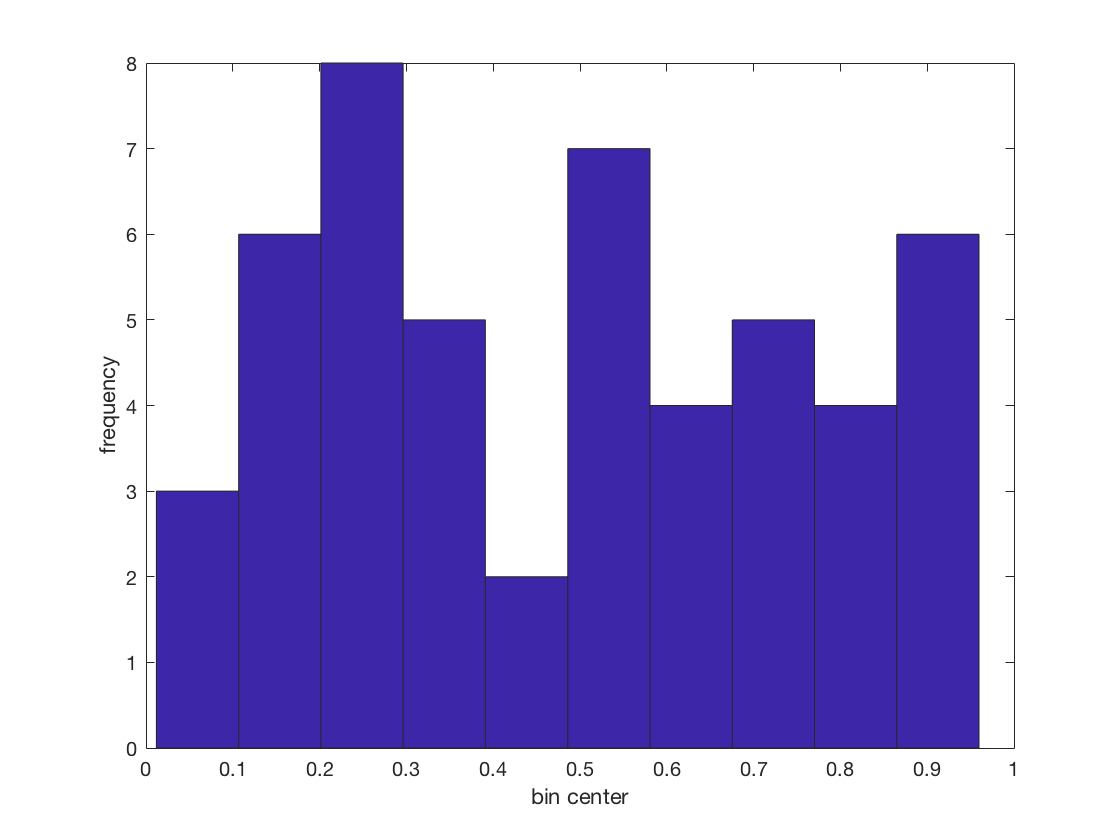
\includegraphics[width=0.6\linewidth]{5_plot1.png}
	\caption{histogram for $N=50$}
	\label{5_plot1}
\end{figure}

With a sample size $N=500$ we get $\mu=0.4862$ and $\sigma=0.2898$, which is fairly close to the theoretical values, though the $\mu$ value is actually further from the theoretical value than when $N=50$. See figure \ref{5_plot2}, below, for a histogram of the experimental values. From the histogram we can see that the actual distribution of values is more uniform than in the previous case, though it still has distinct peaks that one would not expect with a truly uniform distribution.

\begin{figure}[h!]
	\centering
	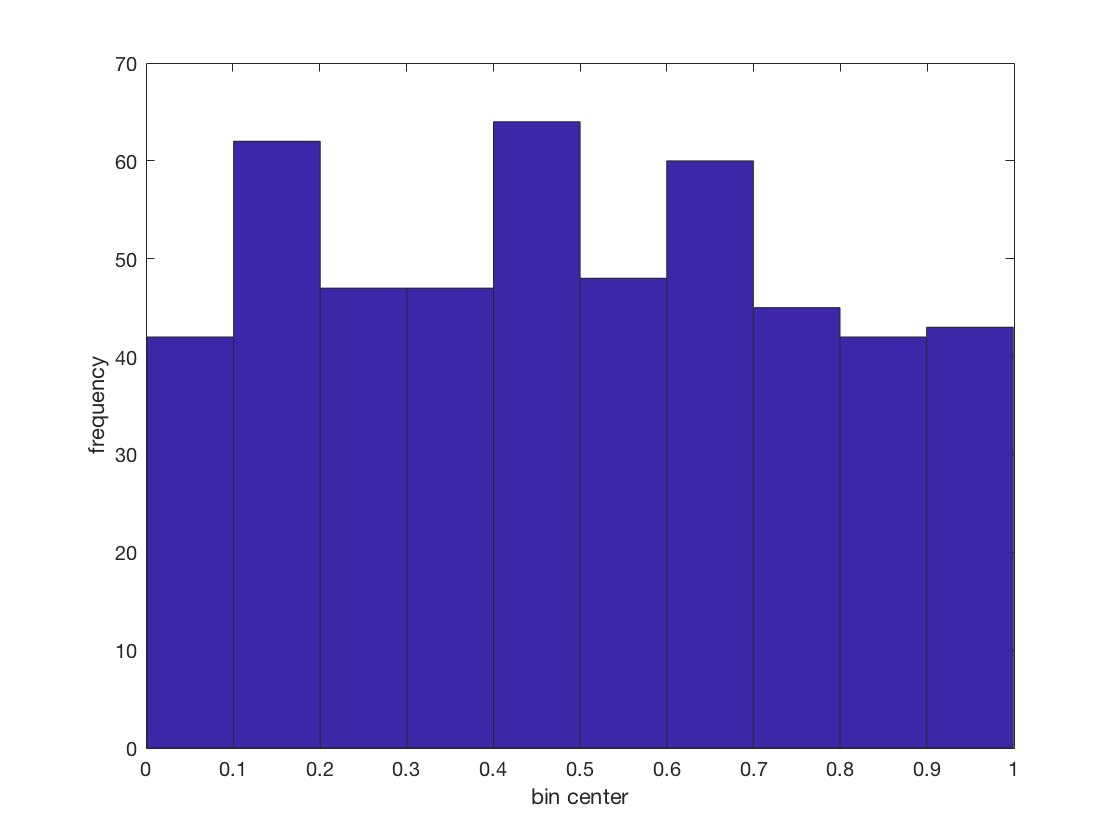
\includegraphics[width=0.6\linewidth]{5_plot2.png}
	\caption{histogram for $N=500$}
	\label{5_plot2}
\end{figure}

With a sample size $N=500$ we get $\mu=0.4999$ and $\sigma=0.2892$, which is nearly the same as the theoretical values. See figure \ref{5_plot3}, below, for a histogram of the experimental values. From the histogram we can see that the actual distribution of values is very nearly uniform, with each of the 10 bins containing about 500 values.

\begin{figure}[h!]
	\centering
	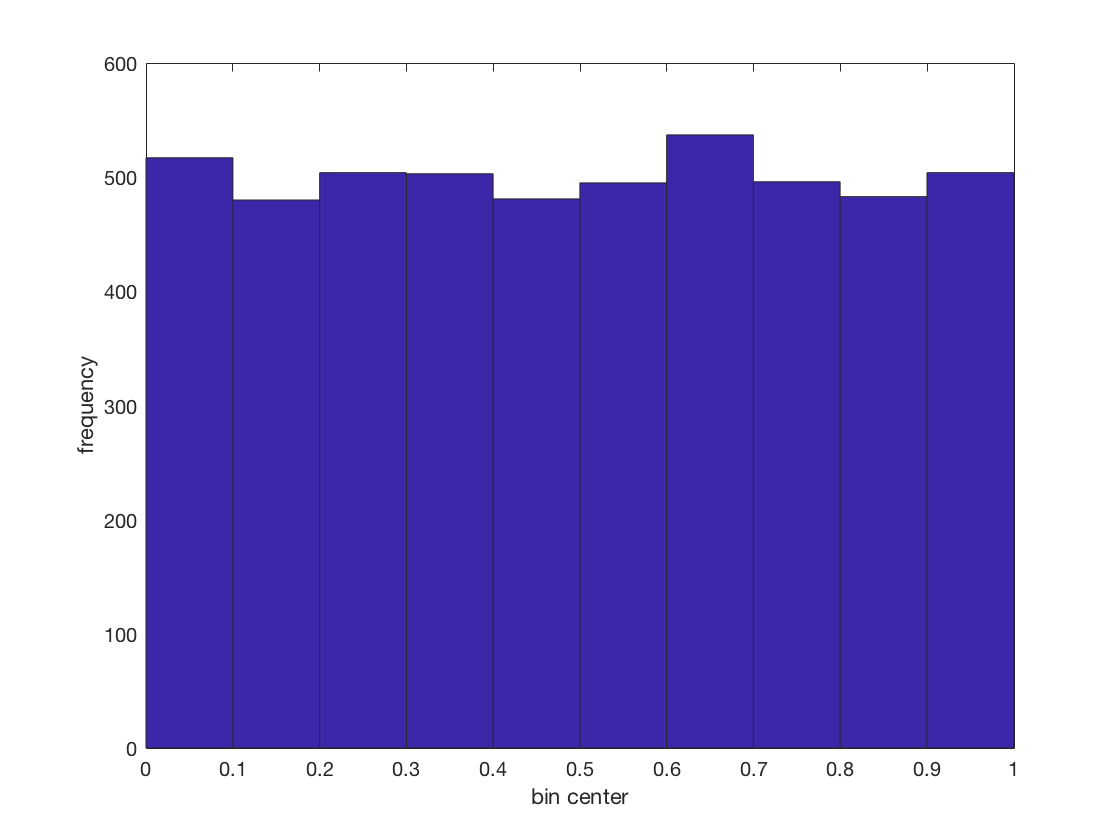
\includegraphics[width=0.6\linewidth]{5_plot3.png}
	\caption{histogram for $N=5000$}
	\label{5_plot3}
\end{figure}

\section*{Exercise 6}
Generate $10000$ samples of $(x_1+x_2)/2$, where each $x_i$ is a random number uniformly distributed on $[-1/2,+1/2]$. Plot the samples in a 50-bin histogram. Repeat for $(x_1+x_2+x_3+x_4)/4$. Describe the difference between the two histograms.

\subparagraph*{}
The plot below shows a histogram for $10000$ samples of $(x_1 + x_2)/2$. Because each value in this distribution is the mean of two samples from a uniform probability distribution one would expect the distribution to be more heavily weighted toward the mean and to taper off linearly as $x$ diverges from the mean. This is exactly what we see in figure \ref{6_plot1}, below.
\begin{figure}[h!]
	\centering
	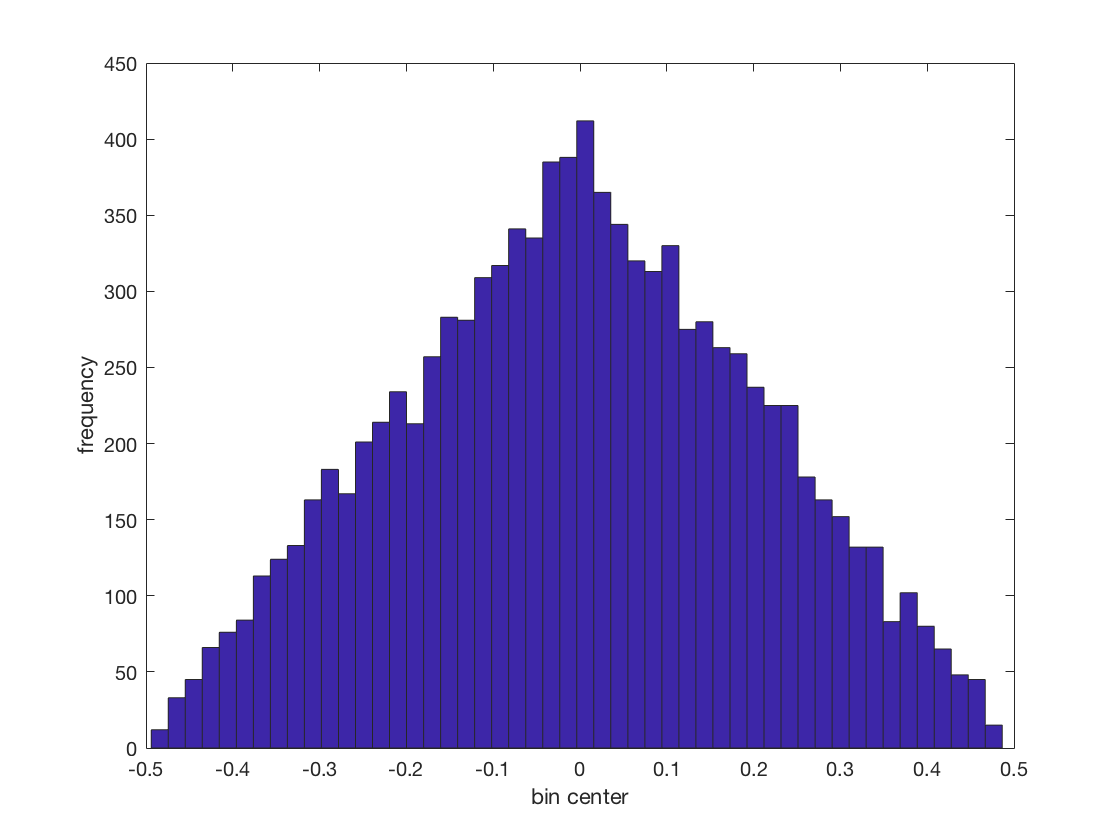
\includegraphics[width=0.6\linewidth]{6_plot1.png}
	\caption{histogram for $(x_1 + x_2)/2$}
	\label{6_plot1}
\end{figure}

The plot below shows a histogram for $10000$ samples of $(x_1 + x_2 + x_3 + x_4)/4$. Because each value in this distribution is the mean of four samples from a uniform probability distribution one would expect the distribution to be more heavily weighted toward the mean as in the previous case. However, instead of tapering linearly we would expect the tapering to approximate a polynomial shape. Again, this is what we see in figure \ref{6_plot2}, below.
\begin{figure}[h!]
	\centering
	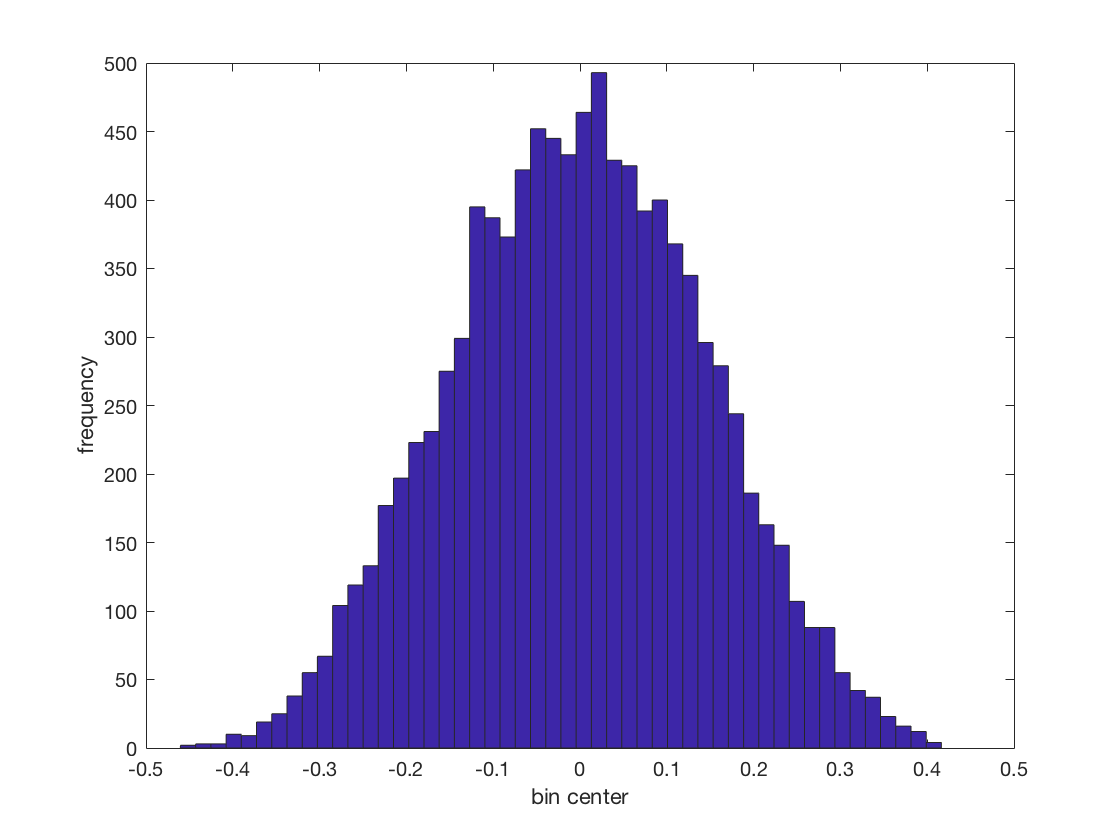
\includegraphics[width=0.6\linewidth]{6_plot2.png}
	\caption{histogram for $(x_1 + x_2 + x_3 + x_4)/4$}
	\label{6_plot2}
\end{figure}

\section*{AQ 1}
Consider the following probability density function:
\begin{equation*}
	f_X(x) = \frac{ab}{b^2+x^2},\quad b>0
\end{equation*}

\subsection*{Problem (a)}
Determine the value of a in the pdf so that $f_X(x)$ is a valid probability density function. Note: the correct value of $a$ makes $f_X(x)$ a Cauchy pdf.

\subparagraph*{}
Knowing $\int_{-\infty}^\infty f_X(x)dx = 1$ we can find $a$ via the following:
\begin{align*}
	1 &= \int_{-\infty}^\infty \frac{ab}{b^2+x^2}dx \\
	&= ab\int_{-\infty}^\infty \frac{1}{b^2 + x^2}dx \\
	&= ab\Bigg[\frac{1}{b}\tan^{-1}\frac{x}{b}\Bigg|_{-\infty}^\infty \\
	&= a\tan^{-1}\frac{x}{b}\Bigg|_{-\infty}{\infty} \\
	&= \frac{a\pi}{2}  + \frac{a\pi}{2} \\
	&= a\pi \\ 
	a &= \frac{1}{\pi}
\end{align*}

\subsection*{Problem (b)}
Find the mean of a Cauchy random variable.

\section*{AQ 2}

\end{document}
